\documentclass[a4paper]{article}

\usepackage[margin=1.25in]{geometry}
\usepackage{fancyhdr}
\usepackage{enumitem}
\usepackage{tabularx}
\usepackage{float}
\usepackage{subcaption}
\usepackage{array}
\usepackage{graphicx}

\usepackage[hidelinks]{hyperref}
\hypersetup{
    colorlinks=true,
    linkcolor=blue,
    filecolor=blue}

\begin{document}

\begin{titlepage}
    \thispagestyle{fancy}
    \renewcommand{\headrulewidth}{0pt}
    \begin{center}
        \vspace*{2cm}

        \LARGE\textbf{University of North Carolina at Charlotte\\
                        Department of Electrical and Computer Engineering}
        
        \vspace*{4cm}

        Homework Report $\# 4$ \\
        \Large\textbf{ECGR 4106 - Real-Time Machine Learning} \\
        
        \noindent\rule{14cm}{0.4pt}

        \vspace*{3cm}

        Name: Govind Menon \\
        Student ID: 801371478 \\
        Date: July 8, 2026 \\
        GitHub: \href{https://github.com/pGovm/introToDL.git}{pGovM/introToDL}

    \end{center}
\end{titlepage}

\section{\textbf{\textbf{Hyper Parameters}}}
These hyperparameters were shared in all 3 problems 

\begin{itemize}
    \item Hidden Size: 128
    \item Epochs: 50
    \item Learning Rate: 1e-4
    \item Maximum Length of Sentence: 100
    \item Batch Size: 1 (problems 3 \& 4), 16 (problems 1 \& 2)
    \item Train/Val Split: 80/20
    \item Random Seed: 42
\end{itemize}

\section*{\textbf{Problem 1}}
\textbf{Objective}: Train and validate a transformer model for learning the given sequence, with sequence lengths of 10, 20, and 30. Report and compare the model metrics against the  RNN-based approach in the previous homework.

\begin{figure}[H]
    \centering
    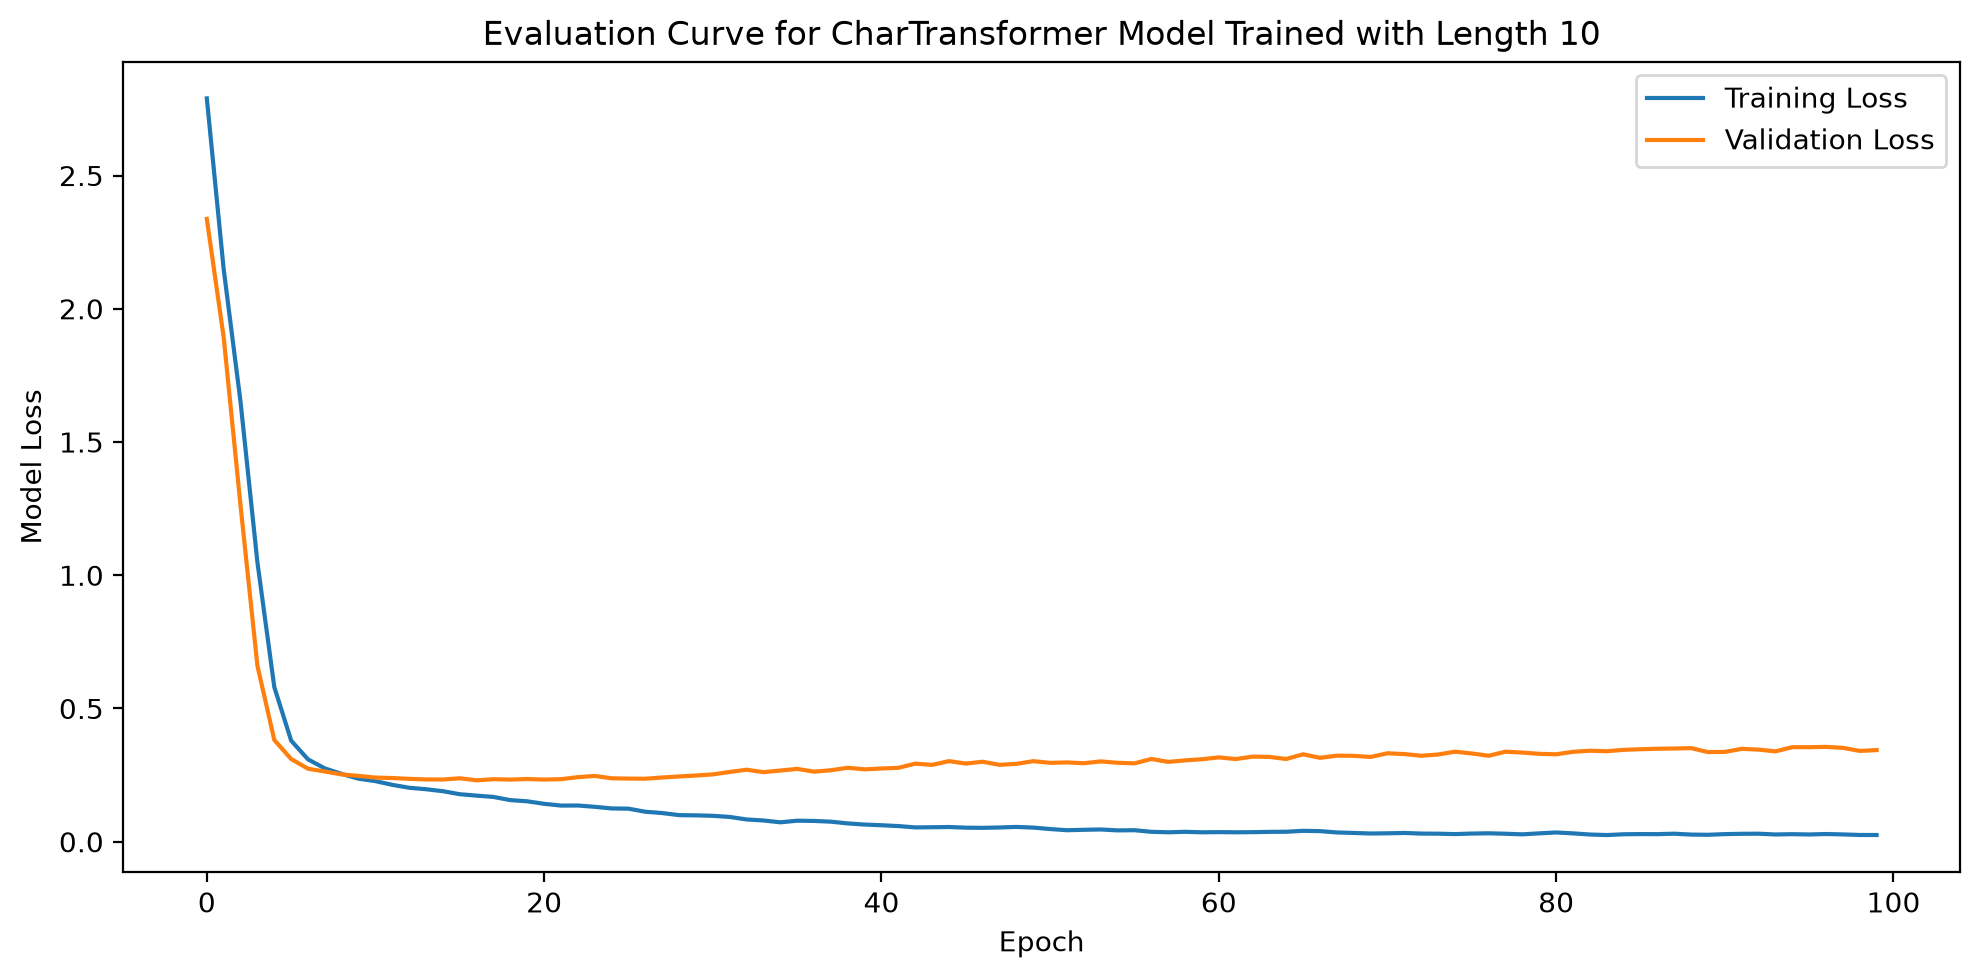
\includegraphics[width=\linewidth]{../../hw4/output/p1/charTransformer_len10_evalCurve.png}
    \caption{\textbf{Evaluation Curves for Transformer Model Trained with Sequence Length of 10}}
    \label{fig:transLen10evalCurve}
\end{figure}

\begin{figure}[H]
    \centering
    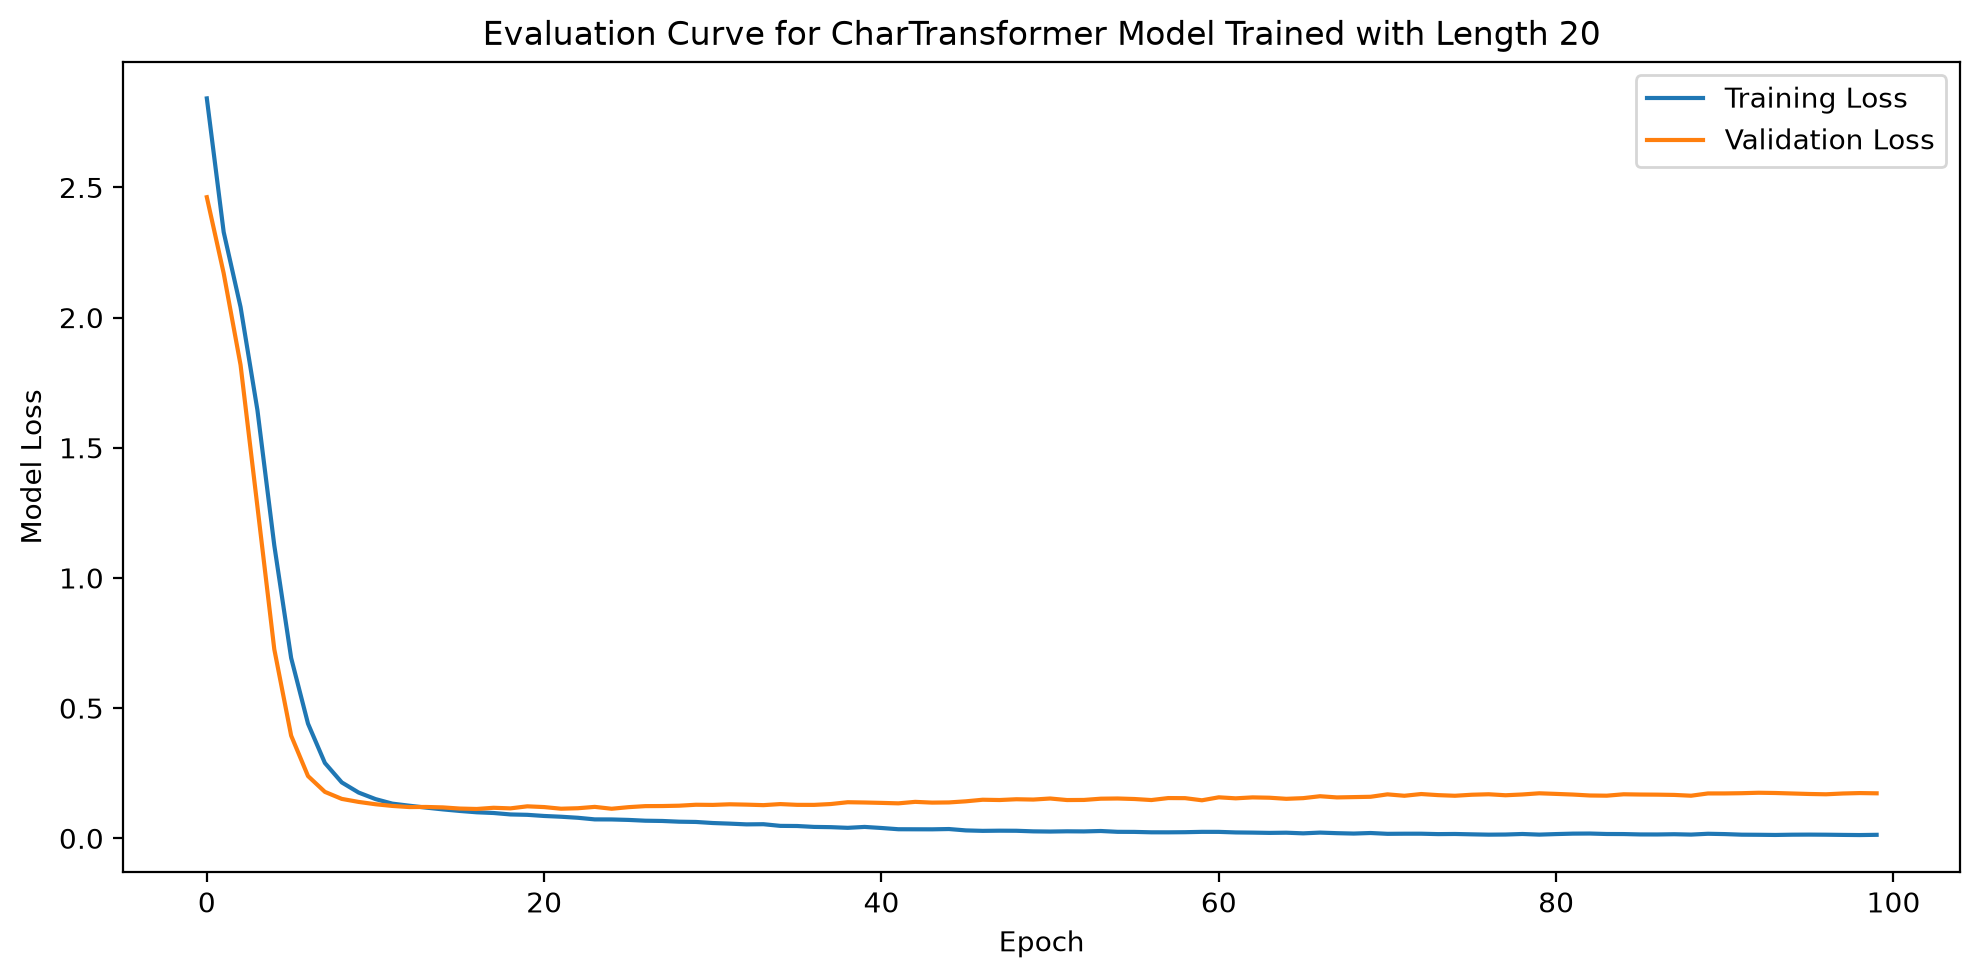
\includegraphics[width=\linewidth]{../../hw4/output/p1/charTransformer_len20_evalCurve.png}
    \caption{\textbf{Evaluation Curves for Transformer Model Trained with Sequence Length of 20}}
    \label{fig:transLen20evalCurve}
\end{figure}

\begin{figure}[H]
    \centering
    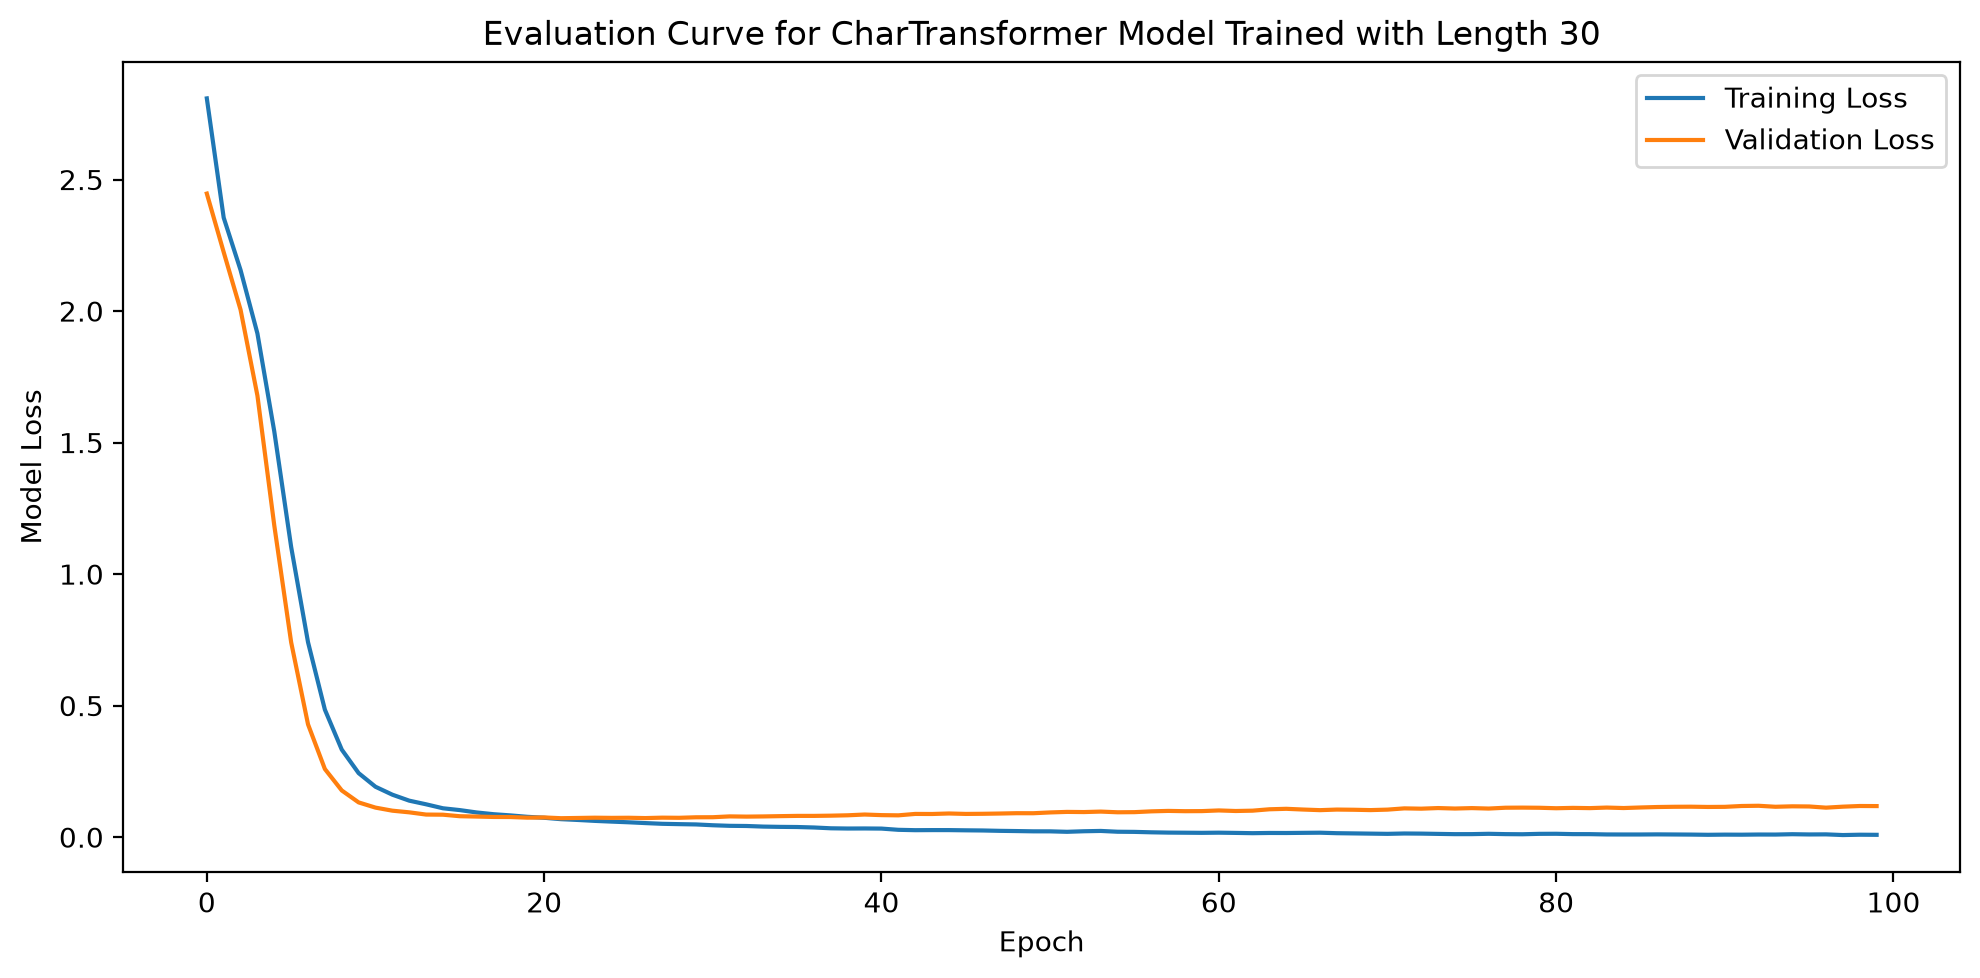
\includegraphics[width=\linewidth]{../../hw4/output/p1/charTransformer_len30_evalCurve.png}
    \caption{\textbf{Evaluation Curves for Transformer Model Trained with Sequence Length of 30}}
    \label{fig:transLen30evalCurve}
\end{figure}



\subsection*{Training Loss}

\begin{table}[H]
    \centering
    \caption{\textbf{Final Training Loss }}
    \label{tab:finalTLp1}
    \begin{tabular}{| c || c | c | c | c |}
        \hline
        Sequence Length \ Model & \textbf{Transformer} & \textbf{RNN} & \textbf{LSTM} & \textbf{GRU} \\
        \hline
        \textbf{10} & 0.1215 & 0.0906 & 0.0888 & 0.0630 \\
        \hline
        \textbf{20} & 0.0965 & 0.1039 & 0.1566 & 0.0992 \\
        \hline
        \textbf{30} & 0.0634 & 0.1126 & 0.1592 & 0.0419 \\
        \hline
    \end{tabular}
\end{table}

\subsection*{Validation Loss}

\begin{table}[H]
    \centering
    \caption{\textbf{Final Validation Loss}}
    \label{tab:finalVLp1}
    \begin{tabular}{| c || c | c | c | c |}
        \hline
        Sequence Length \ Model & \textbf{Transformer} & \textbf{RNN} & \textbf{LSTM} & \textbf{GRU} \\
        \hline
        \textbf{10} & 0.2249 & 2.540 & 2.557 & 2.571 \\
        \hline
        \textbf{20} & 0.1087 & 2.694 & 2.297 & 2.495 \\
        \hline
        \textbf{30} & 0.0722 & 2.740 & 2.472 & 2.697 \\
        \hline
    \end{tabular}
\end{table}



\subsection*{Validation Accuracy}

\begin{table}[H]
    \centering
    \caption{\textbf{Validation Accuracy (\%)}}
    \label{tab:finalVAp1}
    \begin{tabular}{| c || c | c | c | c |}
        \hline
        Sequence Length \ Model & \textbf{Transformer} & \textbf{RNN} & \textbf{LSTM} & \textbf{GRU} \\
        \hline
        \textbf{10} & 94.35 & 49.26 & 44.86 & 50.73 \\
        \hline
        \textbf{20} & 97.00 & 50.31 & 49.47 & 52.42 \\
        \hline
        \textbf{30} & 97.99 & 47.99 & 47.57 & 49.26 \\
        \hline
    \end{tabular}
\end{table}

\subsection*{Model Complexity}

\begin{table}[H]
    \centering
    \caption{\textbf{Model Complexity (FLOPs)}}
    \label{tab:FLOPsp1}
    \begin{tabular}{| c || c | c | c | c |}
        \hline
        Sequence Length \ Model & \textbf{Transformer} & \textbf{RNN} & \textbf{LSTM} & \textbf{GRU} \\
        \hline
        \textbf{10} & 10.56M & 337.2k & 1.337M & 1.005M \\
        \hline
        \textbf{20} & 21.13M & 668.8k & 2.668M & 2.005M \\
        \hline
        \textbf{30} & 31.69M & 1M & 3.999M & 3.005M \\
        \hline
    \end{tabular}
\end{table}

\subsection*{Number of Parameters}

\begin{table}[H]
    \centering
    \caption{\textbf{No. of Params}}
    \label{tab:Paramsp1}
    \begin{tabular}{| c || c | c | c | c |}
        \hline
        Sequence Length \ Model & \textbf{Transformer} & \textbf{RNN} & \textbf{LSTM} & \textbf{GRU} \\
        \hline
        \textbf{10} & 1.06M & 44.59k & 143.6k & 110.6k \\
        \hline
        \textbf{20} & 1.06M & 44.59k & 143.6k & 110.6k \\
        \hline
        \textbf{30} & 1.06M & 44.59k & 143.6k & 110.6k \\
        \hline
    \end{tabular}
\end{table}

\subsection*{Model Size}

\begin{table}[H]
    \centering
    \caption{\textbf{Model Size (MB)}}
    \label{tab:MBp1}
    \begin{tabular}{| c || c | c | c | c |}
        \hline
        Sequence Length \ Model & \textbf{Transformer} & \textbf{RNN} & \textbf{LSTM} & \textbf{GRU} \\
        \hline
        \textbf{10} & 7.0099 & 0.1701 & 0.5480 & 0.4220 \\
        \hline
        \textbf{20} & 7.0099 & 0.1701 & 0.5480 & 0.4220 \\
        \hline
        \textbf{30} & 7.0099 & 0.1701 & 0.5480 & 0.4220 \\
        \hline
    \end{tabular}
\end{table}

\subsection*{Training Time}

\begin{table}[H]
    \centering
    \caption{\textbf{Training Time (s)}}
    \label{tab:trainTp1}
    \begin{tabular}{| c || c | c | c | c |}
        \hline
        Sequence Length \ Model & \textbf{Transformer} & \textbf{RNN} & \textbf{LSTM} & \textbf{GRU} \\
        \hline
        \textbf{10} & 7.0099 & 0.56 & 1.10 & 0.79 \\
        \hline
        \textbf{20} & 7.0099 & 0.41 & 1.76 & 1.22 \\
        \hline
        \textbf{30} & 7.0099 & 0.63 & 2.37 & 1.70 \\
        \hline
    \end{tabular}
\end{table}

\section*{\textbf{Problem 2}}
\textbf{Objective}: Build a transformer model for the tiny Shakespeare dataset with sequence lengths of 20, 30, and 50 while exploring transformer architectures with 1, 2, and 4 transformer blocks, combined with 2 and 4 heads. Report the resulting metrics.

\section*{\textbf{Problem 3}}
\textbf{Objective}: Develop a transformer-based encoder-decoder architecture for English-to-French translation, explore the same transformer architectures of 1, 2, and 4 transformer blocks with 2 and 4 heads. Report standard model metrics combined with traditional sequence accuracy and validation bleu-4 score based on the validation set. Compare your best-performing transformer configuration against the Homework 3 RNN-based models, across all the previously mentioned metrics.

\section*{\textbf{Problem 4}}
\textbf{Objective}: Repeat the same exercise as problem 3 but translate from French to English using the same dataset.

\end{document}
